\section{Overall dephasing rate}
\label{sec3}

A periodic drive mitigates low-frequency flux-induced dephasing by coupling the FTT states and suppressing the first-order sensitivity of the dressed cavity frequency to fluctuations of $\omega_b$. However, the drive also contributes new dephasing channels when FTT relaxation is present.

To quantify the total cavity dephasing rate, the system is modeled with a stochastic master equation. For a given flux-noise realization $\delta\Phi(t)$, the density matrix $\rho(t)$ obeys
\begin{align}
\dot{\rho}
&= -i\left[\,H_{\mathrm{sys}} + \delta\omega_b(t)\, b^\dagger b,\ \rho\,\right]
+ \gamma_{b\downarrow}\,\mathcal{D}[b]\rho,
\nonumber \\
H_{\mathrm{sys}}
&= H_{\mathrm{static}} + 2\Omega_0 \cos(\omega_d t)\,(b + b^\dagger).
\label{Linblad}\end{align}
Here $\mathcal{D}[b]\rho = b\rho b^\dagger - \tfrac{1}{2}\{b^\dagger b, \rho\}$ describes FTT relaxation at rate $\gamma_{b\downarrow}$ (the FTT energy-relaxation rate).

Flux noise in these devices typically exhibits a $1/f$ spectrum. The corresponding power spectral density is taken as
\begin{equation}
S_{1/f}(\omega)
= \int_{-\infty}^{\infty} d\tau\, \langle \delta\Phi(\tau)\,\delta\Phi(0)\rangle\, e^{i\omega \tau}
= \frac{S_0^{\,2}}{\left|\omega/2\pi\right|},
\end{equation}
where $S_0$ sets the flux-noise amplitude.

The following analysis is carried out in the effective-drive frame to separate the roles of relaxation and dephasing. The unselective and selective regimes are treated in turn.
\subsection{Total dephasing in the unselective regime}
\label{subsec:unselective-dephasing}

In the unselective regime $|\Delta_{bd}|\gg|\chi|$, the master equation can be expanded to first order in $|\chi/\Delta_{bd}|$ about the sweet-spot condition (Eq.\ \eqref{eq:ss_unselective}). This yields the Lindblad master equation for the density matrix in the effective drive frame $\rho_d$,
\begin{align}
\label{eq:Ldiss_unselective}
&\dot{\rho}_d = -i \bigl[ H_d + H_{\text{noise}}^d , \rho_d \bigr] \nonumber 
+ \widetilde{\gamma}_{b\downarrow}^{\mathrm{un}} \mathcal{D}[\sigma^-]\rho_d
+ \gamma_{b\uparrow}^{\mathrm{un}} \mathcal{D}[\sigma^+]\rho_d\\
+ &2\gamma_{c\phi}^{\mathrm{un}} \mathcal{D}[c^\dagger c]\rho_d
+ \widetilde{\gamma}_{c\downarrow}^{\mathrm{un}} \mathcal{D}[c]\rho_d,
\end{align}
See App.~\ref{Linbladian regime} for the derivation.
The effective rates $\widetilde{\gamma}_{b\downarrow}^{\mathrm{un}}$, $\gamma_{b\uparrow}^{\mathrm{un}}$, $\gamma_{c\phi}^{\mathrm{un}}$, and $\widetilde{\gamma}_{c\downarrow}^{\mathrm{un}}$ are given below.
Here, $H_d$ is the effective driven Hamiltonian Eq.\ \eqref{eq:Hd_far_detuned}, and $H_{\text{noise}}^d$ is the noise Hamiltonian in the effective-drive frame. In the unselective limit it takes the approximate form
\begin{align}
\label{eq:Hnoise_unselective}
H_{\text{noise}}^d &\approx \delta \omega_b \Bigg[ \big(1- \frac{\Delta_{bd}}{2K}\big) \sigma^+ \sigma^- \nonumber+ \frac{2 g^2}{\Delta_{bc}^2} \left( 1 - \frac{2 K}{\Delta_{bc}} \right) \sigma^+ \sigma^- c^\dagger c  
\\
&-\frac{1}{2} \sqrt{\frac{\Delta_{bd}}{K}} \sigma_x \Bigg].
\end{align}
Although the sweet-spot condition cancels the leading direct cavity-dephasing contribution (\(D_{0\to1}=0\)), it does not eliminate all noise channels in the effective-drive frame, which are discusseed below.
\paragraph{Interpretation of the dissipators.}
The dissipators in Eq.~\eqref{eq:Ldiss_unselective} represent (i) drive-renormalized FTT relaxation,
$\widetilde{\gamma}_{b\downarrow}^{\mathrm{un}}\mathcal{D}[\sigma^-]$; (ii) drive-induced FTT excitation,
$\gamma_{b\uparrow}^{\mathrm{un}}\mathcal{D}[\sigma^+]$, which produces photon-shot-noise dephasing of the cavity via the dispersive coupling \cite{shotnoise,PhysRevA.75.042302Ashphotonshot}; (iii) cavity pure dephasing,
$2\gamma_{c\phi}^{\mathrm{un}}\mathcal{D}[c^\dagger c]$ (the prefactor $2$ is conventional); and (iv) renormalized cavity decay,
$\widetilde{\gamma}_{c\downarrow}^{\mathrm{un}}\mathcal{D}[c]$.
At the sweet-spot condition of Eq.~\eqref{eq:ss_unselective}, the corresponding rates are
\begin{align}
\widetilde{\gamma}_{b\downarrow}^{\mathrm{un}}
&= \gamma_{b\downarrow}\left(1-\frac{\Delta_{bd}}{K}\right), \nonumber\\
\gamma_{b\uparrow}^{\mathrm{un}}
&= \frac{\gamma_{b\downarrow}}{16}\left(\frac{\Delta_{bd}}{K}\right)^2
\left(1-\frac{2\Delta_{bd}}{K}\right), \nonumber\\
\gamma_{c\phi}^{\mathrm{un}}
&= \frac{1}{2}\gamma_{b\downarrow}\left(\frac{g}{\Delta_{bc}}\right)^4\frac{K}{\Delta_{bd}}, \qquad
\widetilde{\gamma}_{c\downarrow}^{\mathrm{un}}
= \gamma_{c\downarrow}\left(1+\frac{g^2}{\Delta_{bc}^2}\right).
\end{align}
The cavity-decay renormalization scales as $g^2/\Delta_{bc}^2$ and remains small (e.g., $\sim 0.01$) even in the relatively strong dispersive-coupling regime.

\paragraph{Interpretation of the noise Hamiltonian.}
At the sweet spot, cavity dephasing $c^\dagger c$ in Eq.~\eqref{eq:Hnoise_unselective} vanishes by construction , suppressing direct cavity-frequency noise. Also, AC-Stark-shift-induced cavity-frequency fluctuations are neglected because the FTT is barely excited if it is initialized in the ground state. Residual dephasing is dominated by a transverse component $\propto\sigma_x$, which induces FTT depolarization under $1/f$ flux noise. The transverse-noise-induced excitation rate is
\begin{equation}
\gamma_{b\uparrow}^{1/f,\mathrm{un}}=\left(\frac{\Omega_0}{\Delta_{bd}}\frac{\partial\omega_b}{\partial\Phi}\right)^2\frac{S_0^2}{|\Delta_{bd}/2\pi|}
\overset{\eqref{eq:ss_unselective}}{=}\frac{1}{4}\left(\frac{\partial\omega_b}{\partial\Phi}\right)^2\frac{S_0^2}{|K/2\pi|}
\end{equation}
at the sweet-spot condition.

\paragraph{Total cavity dephasing rate.}
In the unselective regime, evaluated at the sweet spot, the total cavity dephasing rate is the sum of the three contributions in \begin{align}
\label{eq:Gamma_phi_total_unselective}
&\Gamma_{\phi,\mathrm{total}}
=\gamma_{b\uparrow}^{1/f,\mathrm{un}}+\gamma_{b\uparrow}^{\mathrm{un}}+\gamma_{c\phi}^{\mathrm{un}} \nonumber\\
&=\left(\frac{\partial\omega_b}{\partial\Phi}\right)^2\frac{S_0^2}{4K}
+\frac{\gamma_{b\downarrow}}{16}\left(\frac{\Delta_{bd}}{K}\right)^2\bigg(1-\frac{2\Delta_{bd}}{K}\bigg)\nonumber
\\&+\frac{\gamma_{b\downarrow}}{2}\left(\frac{g}{\Delta_{bc}}\right)^4\frac{K}{\Delta_{bd}}.
\end{align}
We approximate the photon-shot-noise contribution to cavity dephasing by the FTT heating rate $\gamma_{b\uparrow}^{\mathrm{un}}$ in the limit $\chi \gg \widetilde{\gamma}_{b\downarrow}$ \cite{serge}, because a single photon event is sufficient to entirely destroy phase coherence before the photon decays. Under this approximation, each contribution in Eq.~\eqref{eq:Gamma_phi_total_unselective} agrees well with numerical simulations, as verified in App.~\ref{app:dephasing_unselective}. We also emphasize that the drive induces only a small correction to $\gamma_{c\downarrow}$, scaling as $g^2/\Delta_{bc}^2 \ll 1$; see App.~\ref{app:dephasing_unselective}.
\subsection{Total dephasing in the selective regime}
\label{subsec:total_dephasing_selective}

Operating at the selective-regime sweet spot protects the cavity states
$\lvert g,m^\star\rangle$--$\lvert g,m^\star\!+\!1\rangle$ from flux-noise dephasing.
Under drive, however, the residual dephasing budget in the selective regime is set by two
contributions: (i) cavity pure dephasing at a rate
$\gamma_{c\phi}^{\mathrm{sel}}=\bigl(g^2/\Delta_{bc}^2\bigr)\gamma_{b\downarrow}$,
arising from the Purcell-like mixing of cavity and FTT decay channels, and
(ii) FTT heating at a rate $\gamma_{b\uparrow}^{\mathrm{sel}}\propto 1/\lvert\Delta_{bd}\rvert$
induced by photon shot noise (see App.~\ref{Linbladian regime} for derivations). Because the shot-noise contribution scales unfavorably as $1/\lvert\Delta_{bd}\rvert$, operating at larger detuning—i.e., in the unselective regime—yields a lower total dephasing rate.

\subsection{Numerical evaluation of the total dephasing rate}
\label{subsec:numerical_total_dephasing_rate}

Full-system simulations are used to extract the cavity dephasing rate under drive; the
numerical procedure and fitting protocol are summarized in App.~\ref{app:dephasing_numerics}.
The noise amplitude $S_0$ and the detuning $\Delta_{bd}$ are sampled over the parameter
range of interest. For each $\Delta_{bd}$, the drive amplitude is chosen to satisfy the
sweet-spot condition, and the corresponding total dephasing rate
$\Gamma_{\phi,\mathrm{total}}$ is extracted.

Fig.~\ref{fig:total_rate}(a) summarizes the results. For $S_0=10^{-5}/\Phi_0$, the
drive-induced contribution $\gamma_{b\uparrow}^{1/f,\mathrm{un}}$ dominates
$\Gamma_{\phi,\mathrm{total}}$ over the scanned detuning range. At large detuning,
$\lvert\Delta_{bd}\rvert> \lvert\chi\rvert\simeq 2~\mathrm{MHz}$, the total rate is well described by $\gamma_{b\uparrow}^{1/f,\mathrm{un}}$, which is independent of the detuning. At smaller detuning, i.e.\
$-\Delta_{bd}/2\pi=1~\mathrm{MHz}<\lvert\chi/2\pi\rvert$, the rate
increases as the dynamics enters the selective regime, consistent with the
$1/\lvert\Delta_{bd}\rvert$ scaling.

For smaller noise amplitude, e.g.\ $S_0=10^{-6}/\Phi_0$, the $S_0$-independent drive-induced contributions
$\gamma_{b\uparrow}^{\mathrm{un}}$ and $\gamma_{c\phi}^{\mathrm{un}}$ dominate
$\Gamma_{\phi,\mathrm{total}}$. At large detuning ($-\Delta_{bd}/2\pi=19~\mathrm{MHz}$),
$\gamma_{b\uparrow}^{\mathrm{un}}\propto(\Delta_{bd}/K)^2$ dominates while
$\gamma_{c\phi}^{\mathrm{un}}\sim K/\Delta_{bd}$ is suppressed; the opposite hierarchy
holds at small detuning ($-\Delta_{bd}/2\pi=1~\mathrm{MHz}$). Consequently,
$-\Delta_{bd}/2\pi=6~\mathrm{MHz}$ yields the minimal $\Gamma_{\phi,\mathrm{total}}$
within the scanned range. In the undriven case, the dephasing time is
$\sim 0.1$--$1~\mathrm{ms}$ as $S_0$ varies from $10^{-5}/\Phi_0$ to $10^{-6}/\Phi_0$. With $\Delta_{bd}/2\pi\simeq -6~\mathrm{MHz}$ and
sweet-spot driving, the dephasing time improves by up to $\sim 20\times$ across the
considered $S_0$ range, confirming the overall dephasing enhancement.

\begin{figure}[t]
    \centering
    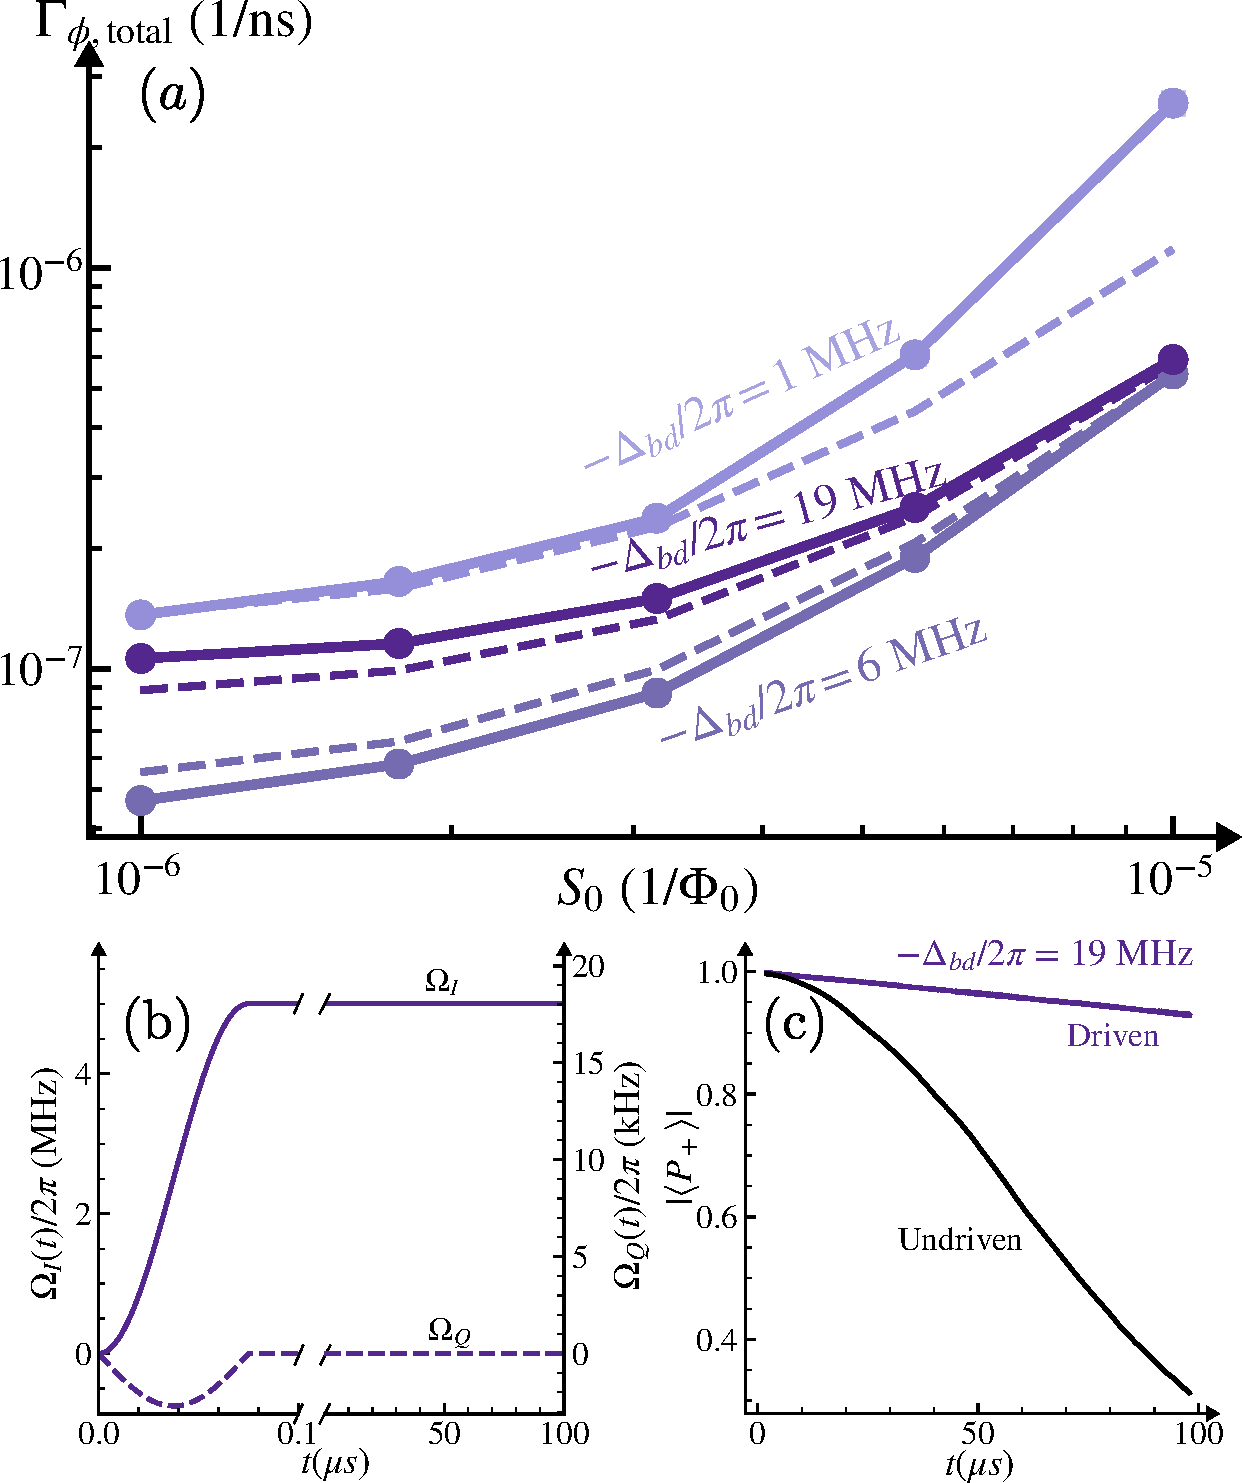
\includegraphics[width=\linewidth]{Sec 3/total_rate.pdf}
    \caption{Numerical evaluation and time-domain validation of the total cavity dephasing
    rate under sweet-spot driving. (a) Total dephasing rate $\Gamma_{\phi,\mathrm{total}}$
    extracted from full-system simulations as a function of detuning $\Delta_{bd}$, with
    the drive amplitude chosen at each detuning to satisfy the sweet-spot condition.
    $S_0$ denotes the amplitude of $1/f$ flux noise. (b) DRAG-style adiabatic ramp pulse.
    (c) Time-domain decay of
$P_X(t)=\mathrm{Tr}\!\left[\rho(t)\,X(t)\right]$, with
$X(t)=\ket{\phi_{g,1}(t)}\!\bra{\phi_{g,0}(t)}+\mathrm{H.c.}$.
The time-dependent Floquet states are labeled by their bare-state correspondence.
The driven system exhibits a cavity dephasing time of $\sim 2~\mathrm{ms}$,
compared to $\sim 100~\mu\mathrm{s}$ in the undriven case.}
    \label{fig:total_rate}
\end{figure}

To visualize the dephasing enhancement directly, we perform time-domain simulations that
include relaxation and stochastic flux noise with $S_0=10^{-5}/\Phi_0$. The initial state is
$\ket{\psi_0}=\tfrac{1}{\sqrt{2}}\big(\ket{g,0}+\ket{g,1}\big)$. With drive, the state is
adiabatically mapped onto the target Floquet states using a shaped pulse
$2\Omega_0(t)\cos\!\big(\omega t+\phi(t)\big)$. In the rotating frame this yields the
$I$ and $Q$ quadratures
\begin{align}
\Omega_I(t) = \Omega(t)\cos\phi(t), \qquad
\Omega_Q(t) = \Omega(t)\sin\phi(t).
\end{align}
We implement a DRAG correction,
$\Omega_Q(t) = -\dot{\Omega}_I(t)/\Delta_{bd}$, which accelerates the adiabatic transfer
relative to $\Omega_I(t)$-only ramps (see App.~\ref{Adiabatic transition}). A pulse ramp
with $\tau=75~\mathrm{ns}$ is shown in Fig.~\ref{fig:total_rate}(b).

The dephasing is quantified by the coherence operator
\begin{align}
X(t) &= \ket{\phi_{g,1}(t)}\!\bra{\phi_{g,0}(t)} + \mathrm{H.c.}, \\
P_X(t) &= \mathrm{Tr}\!\left[\rho(t)\,X(t)\right],
\end{align}
where $\ket{\phi_{g,1}(t)}$ and $\ket{\phi_{g,0}(t)}$ are adiabatically mapped from the bare states.
Without drive, \(1/f\) noise produces sub-Gaussian free-induction decay. At the driven sweet spot, the dominant residual channel is Markovian, arising from FTT depolarization, and yields the exponential decay observed in Fig.~\ref{fig:total_rate}(c). The dephasing time \(T_2\) is extracted from an exponential fit to \(P_X(t)\) (see Appendix I). Under sweet-spot driving, the dephasing time reaches \(\sim 2~\mathrm{ms}\), compared with \(\sim 100~\mu\mathrm{s}\) in the undriven case.